\chapter{Тройное сальто назад можешь? Трюки и фишечки}
\label{ch:tricks}

Далее пойдет речь о красивых приёмах игры, которые лучше осваивать не с листа бумаги, а под присмотром и руководством опытного гитариста. Ощутимо могут помочь видеоролики, поэтому не поленитесь и зайдите, например, на Youtube-канал\footnote{От себя: очень рекомендую Youtube-канал <<Гитара с нуля --- уроки игры на гитаре>> \cite{url:guitarFromZero}, как полноценный обучающий курс, построенный по принципу от простого к сложному. Канал <<Нескучный саунд>> \cite{url:funnySound} хорош для тех, кто подкован в музыке стальными подковами. Электрогитаистам стоит обратить внимание на канал <<fredguitarist>> \cite{url:fredguitarist}, предварительно отсеяв замечательные уроки от отвратительных поливаний грязью всех остальных гитаристов} <<Pima Live>> \cite{url:pimalive}.


\section{А чтоб как капелька упала? Флажолет}
\label{ch:tricks:flageolet}

Флажолетом\footnote{Флажолет (старофр. flageolet --- маленькая флейта). На английском флажолет называют string harmonic, а чаще просто harmonic} называется приём, позволяющий <<изъять>> из обычного звука основной тон и часть обертонов. В результате получается весьма необычный звук.

Для начала вспомним структуру звука, издаваемого струной, обратившись к рисунку \ref{fig:tricks:flageolet:nodes}. Заметим, что в помеченных на рисунке серыми кружками точках струны колебания отсутствуют --- это узлы колебаний. Первый обертон имеет один узел на струне, второй --- два, и тд.

\begin{figure}[!ht]
    \centering
    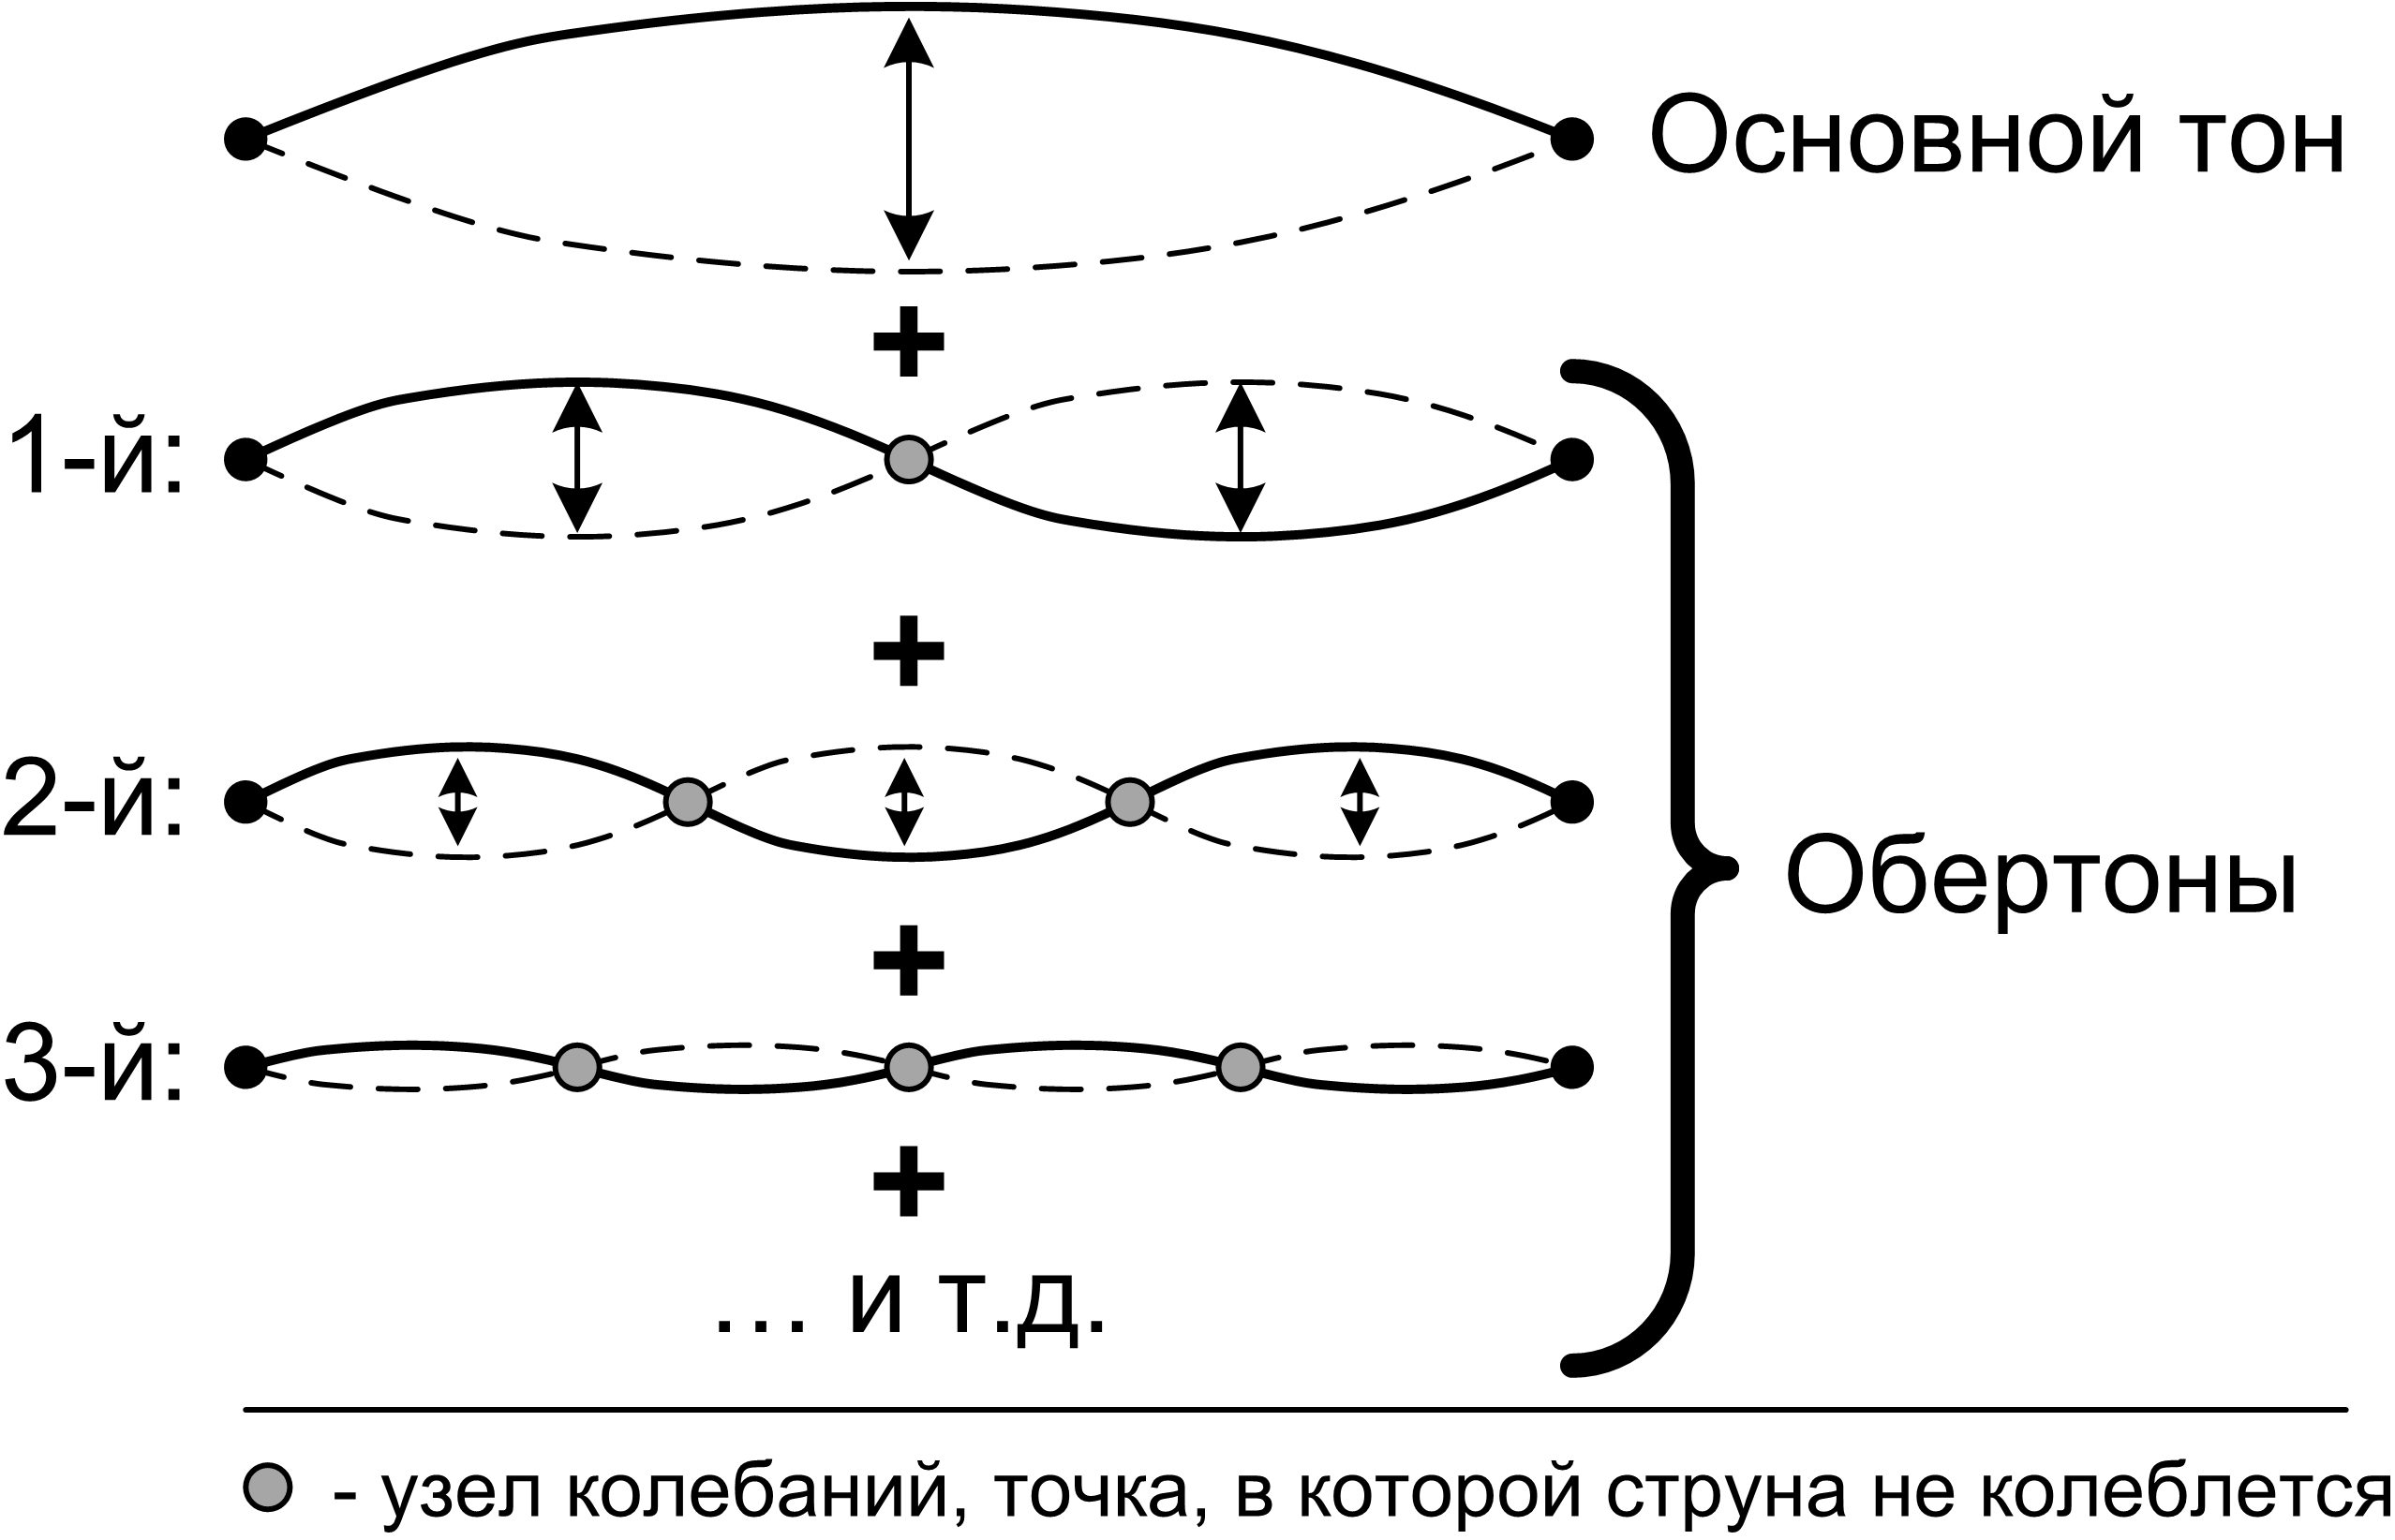
\includegraphics{fig/string-nodes} 
    \caption{Структура звука}\label{fig:tricks:flageolet:nodes}
\end{figure}

\begin{Example}[Сыграем первый флажолет]
    Давайте сыграем флажолет на первой, самой тонкой струне. Там он прозвучит лучше всего. Найдем середину струны --- место, где находится узел первого обертона. Как известно, это прямо над 12-м ладовым порожком. Далее нужно легко поставить палец\footnote{Обычно указательный или средний, какой лучше слушается} левой руки на середину струны, не нужно сильно давить, а тем более прижимать струну к 12-му порожку --- нужно легкое касание. Далее щипните правой рукой струну как обычно, но чуть порезче. Палец левой руки должен уйти с узла вверх на мгновение позже щипка, почти одновременно с ним.
    
    Попробуйте несколько раз, вы поймете, когда у вас получится. Поищите нужное движение, при котором звук получается наиболее ярким.
    
    Причина постоянных неудач: палец левой руки стоит не на узле. 
    
    Если всё получилось, попробуйте сыграть флажолет над 11 или 13-м ладами. Не получается? И не должно. Флажолет --- штука капризная.
    
    Что же получилось в результате извлечения звука таким способом? Палец левой руки заглушил основной тон, а также все обертоны, не имеющие узла в середине струны. Громче всех (вместо основного тона) прозвучит при этом 1-й обертон.
    
    Разница между сыгранным нами флажолетом и обычным щипком на 12 ладу изображена на рисунке \ref{fig:tricks:flageolet:first}.
\end{Example}
 
\begin{figure}[!ht]
    \centering
    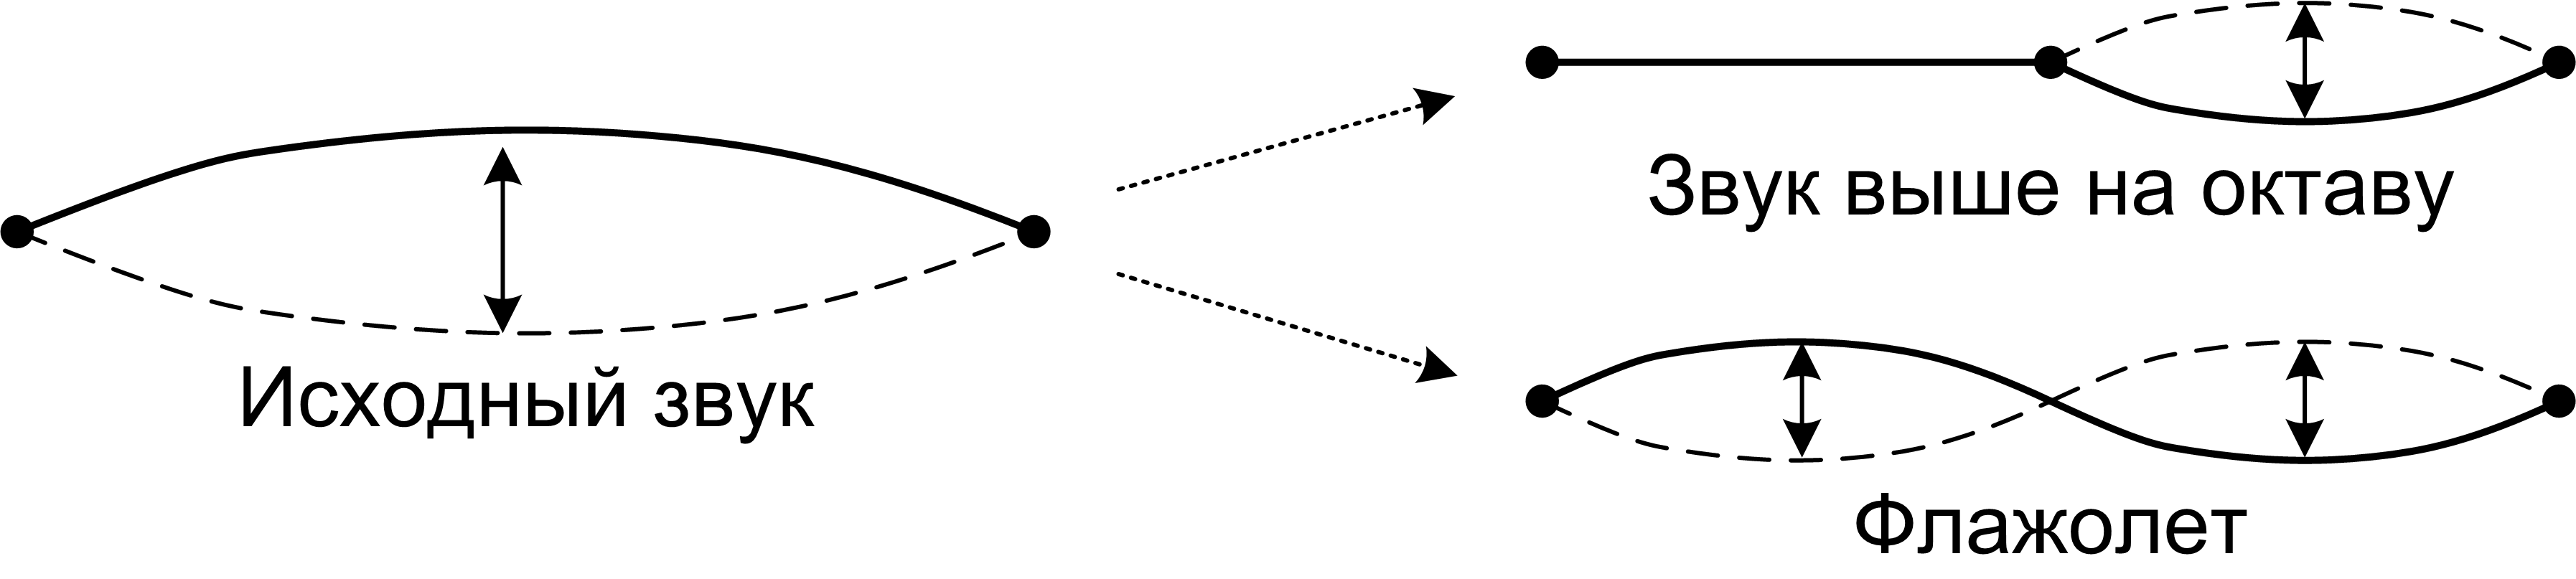
\includegraphics{fig/string-flageolet} 
    \caption{Флажолет первого порядка}\label{fig:tricks:flageolet:first}
\end{figure} 

Этим же приёмом можно сыграть флажолет в узле, делящем струну на три части (см. второй обертон на рисунке \ref{fig:tricks:flageolet:nodes}). В этом случае один из узлов будет находится примерно на 7-м ладу. Давайте это проверим. По формуле \ref{fig:guitar:construction:length} рассчитаем длину звучащего участка струны от нижнего порожка до 7-го лада:
\[
    L(7)=\frac{L}{(\sqrt[12]{2})^7}\approx L\cdot 0.66742
\]

А необходимые нам две трети струны ($\frac{2}{3}\cdot L$) составляют:
\[
    \frac{2}{3}\cdot L \approx L\cdot 0.66667
\]

Абсолютная погрешность будет равна $\Delta \approx 0,00075 \cdot L$. Так как длина струны $L$ на полноразмерной классической гитаре составляет $66$ см., то погрешность составит меньше половины миллиметра. Поглядите на свой пухленький пальчик и смело пренебрегайте погрешностью --- ставьте палец левой руки прямо над 7-м ладом.

Играя флажолет на трети струны, вы столкнетесь с еще одним фактором, влияющим на качество звука: флажолет не прозвучит, если правая рука будет щипать струну вблизи второго узла (треть струны от подставки). Поэкспериментируйте. Капризов у флажолета добавилось.

Четверть струны от верхнего порожка (а от нижнего, соответственно $\frac{3}{4}$) находится примерно над 5-м ладовым порожком. Не забывайте о наличии уже трех узлов колебаний, вблизи которых нельзя щипать струну правой рукой.

На этом пожалуй можно остановиться, потому что флажолеты более высоких порядков играть всё сложнее: они звучат всё тише и тише, а вероятность ошибки всё больше и больше.

Мы разобрались с флажолетами на открытых струнах. Музыканты называют их \emph{натуральными} или \emph{естественными}. Так как на практике играют флажолеты в основном на половине струны, и гораздо реже на трети или четверти, то вариантов не слишком-то много.

Представим, что вы зажали струну на первом ладу, и она стала короче. На каком ладу теперь находится половина струны? Правильно, на 13-м! Сомневаетесь --- поиграйте с формулой \ref{fig:guitar:construction:length}. На каком бы ладу вы не зажали струну, её половина будет находится на 12 ладов выше, треть --- на 7, четверть --- на 5. Количество мест, где можно сыграть флажолет, резко возросло.

Это, конечно, здорово, но если мы зажимаем лад левой рукой, то где взять еще одну руку, чтобы <<придерживать>> узел? На открытой струне это делалось левой рукой. Увы, если у вас нет лишней руки, то справляться придется одной правой. Обычно правая рука делает это так: указательным пальцем касается нужного узла, а большим (безымянным или мизинцем, кому как удобнее) играет щипок, практически одновременно с этим снимая с узла указательный палец (прием проще исполнить, если отодвигать от грифа всю кисть, а не один указательный палец). Знакомьтесь: \emph{искуственный} флажолет.

Итак, самые громкие натуральные флажолеты звучат с узлами на 12, 7 и 5 ладу\ldots Знакомые интервалы, не правда ли? Пожалуй, самое время ещё раз задуматься о природе консонансов! Ну и, конечно, самому поискать ответ на давно, я надеюсь, мучивший вас вопрос: <<Почему октава делится именно на 12 частей?!>> Успехов в самообразовании!


\section{А нужен молоток? Hammer-on, Pull-off}

Это прозвучит напыщенно, но извлекать звуки из гитары можно <<одной левой>>.

Суть приёма Hammer-on в том, что по уже звучащей струне палец левой наносит точный и резкий <<молоточковый>>\footnote{Hammer --- англ. молоток. Hammer-on --- буквально <<молотком --- на!>>} удар, резко прижимая её к ладу. Главное гриф не пробить, не переусердствуйте\footnote{Конечно, главное тут --- не сила, а скорость и точность}! Струна очень резко прижимается к ладу и нерастраченная струной энергия преобразуется в новый, более высокий звук. Чем резче и точнее удар пальцем, тем меньше энергопотери струны, тем громче и чище получится новый звук\footnote{На электрогитаре можно нанести удар и по покоящейся струне --- эффект будет. Кстати, игра <<молоточковыми>>, пробивающими струну до лада, ударами пальцев только уже \emph{правой} руки (левая, при этом либо как обычно, зажимает лады, либо исполняет приемы Hammer-on и Pull-off) называется \emph{тэппинг}. Tapping --- англ. tapping out --- постукивание, выстукивание}.

Pull-off исполняется обычно так: два пальца левой руки заранее ставятся на разные лады на одной и той же струне; правая рука обычным образом извлекает звук; палец левой руки, стоящий на более <<высоком>> ладу (то есть прижимающий конец звучащего отрезка струны) резко сдергивает струну\footnote{Pull off --- буквально переводится с английского как <<срыв>>}, освобождая её. При этом струна, которой <<сдергивание>> добавило энергии, удлиняется до лада, на котором стоит второй палец левой руки, и начинает издавать более низкий звук.

Hammer-on и Pull-off --- приёмы \emph{связного} извлечения звуков. На слух, звуки плавно (а чаще быстро и плавно) как бы <<переходят>> друг в друга\footnote{На самом деле просто отсутвтует резкое увеличение громкости следующего звука, которое бывает при игре щипком правой рукой, ну и струна, перестраиваясь на новую частоту, испытывает длящийся какое-то время <<переходный процесс>>, также создающий ощущение <<плавности>>}. Классическая щкола игры на гитаре обычно использует единый термин для <<свзяного>> извлечения звуков: \emph{легато}. Приём Hammer-on, повышающий звук, классики назовут \emph{восходящим} легато, а понижающий звук Pull-off --- \emph{нисходящим} легато\footnote{Legato --- итал. связанно, плавно}. 

Как говорится: <<К волкам попал --- по волчьи вой>>. В общем, каждый называет эти приемы, в зависимости от того, как требует окружение. Названия <<Hammer-on>> и <<Pull-off>> появились позже <<легато>> и являются более модными в настящее время, особенно в среде эстрадных гитаристов, использующих гитары с электрическим усилением звука.


\section{Как выжать слезу? Вибрато}
\label{ch:tricks:vibrato}

Когда звук сыгран правой рукой, а палец левой руки, прижимающий струну примерно посередине между ладовыми порожками, за счет движения запястья и предплечья как бы <<прокатывается>> подушечкой туда-обратно вдоль струны, возникает очень выразительный, рвущий душу на части звук.  

\begin{figure}[!ht]
    \centering
    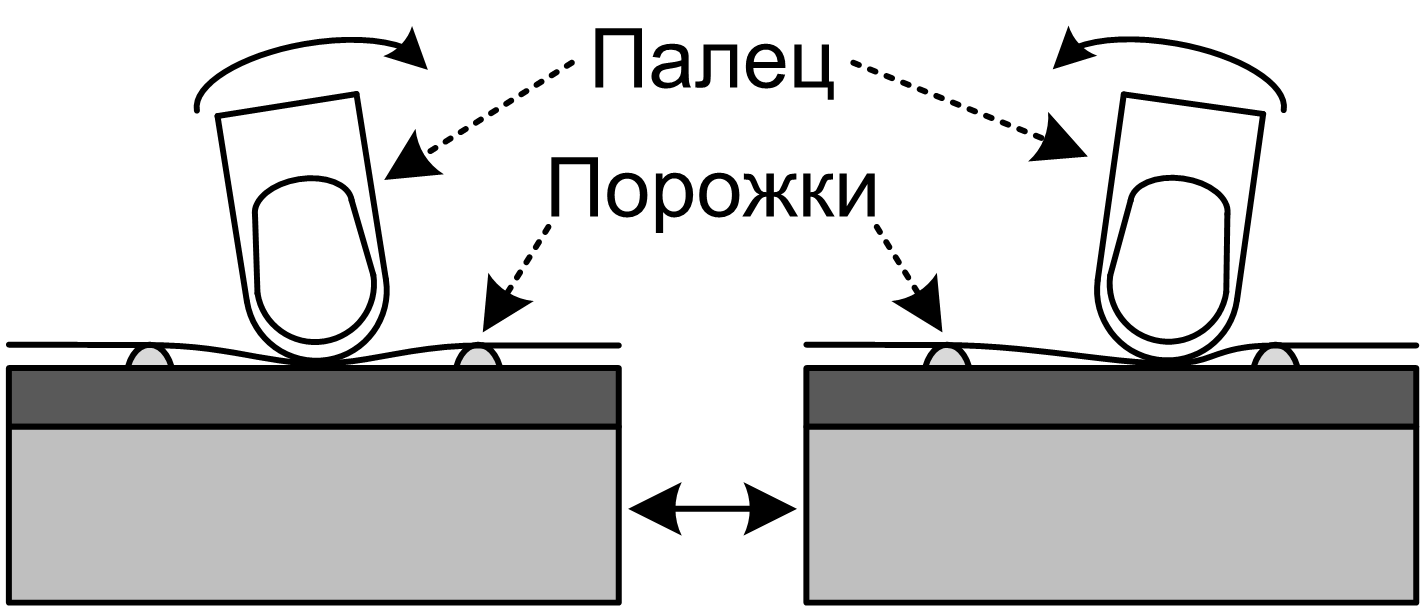
\includegraphics{fig/vibrato} 
    \caption{Приём вибрато}\label{fig:tricks:vibrato}
\end{figure}

Едва уловимые периодические биения высоты основного тона привлекают к себе внимание. Это происходит из-за незначительных изменений натяжения струны, когда по ней прокатывается подушечка пальца. На рисунке \ref{fig:tricks:vibrato} видно, что участок струны между ладами в разных положениях имеет разную длину, а значит из-за этого изменилось и натяжение струны в целом.


\section{Подтяжки? Подтяжка}

О подтяжке мы успели поговорить аж в самом начале. Палец левой ркуи, продолая прижимать звучащую струну к ладу, сдвигает её поперек грифа, как тетиву лука. Натяжение струны при этом сильно меняется, чем достигается куда более сильное повышение высоты звука, чем при вибрато: на полутон а то и на все два. Вариаций подтяжек --- множество, например, можно сначала подтянуть струну, щипнуть, а потом, прижимая к ладу, снять натяжение. 

На английском языке подтяжка называется bend\footnote{Bend --- англ. существительное --- изгиб; глагол --- гнуть, искривлять}. И Русский язык впитал в себя ещё одно заимствование, потому что всё чаще произносят и пишут <<бенд>> вместо <<подтяжка струны>>.
